\documentclass[12pt]{article}

\usepackage[a4paper,margin=2cm]{geometry}

\usepackage{amsmath}
\usepackage{amssymb}
\usepackage{mathtools}

\usepackage{listings}

\usepackage{booktabs} % For tables
\usepackage[table,xcdraw]{xcolor} % For tables

\usepackage{enumerate}
\usepackage{enumitem}

\usepackage{nameref}

\usepackage{xcolor}

\definecolor{codegreen}{rgb}{0,0.6,0}
\definecolor{codegray}{rgb}{0.5,0.5,0.5}
\definecolor{codepurple}{rgb}{0.58,0,0.82}
\definecolor{backcolour}{rgb}{0.95,0.95,0.92}

\lstdefinestyle{mystyle}{
    backgroundcolor=\color{backcolour},
    commentstyle=\color{codegreen},
    keywordstyle=\color{magenta},
    numberstyle=\tiny\color{codegray},
    stringstyle=\color{codepurple},
    basicstyle=\ttfamily\footnotesize,
    breakatwhitespace=false,
    breaklines=true,
    captionpos=b,
    keepspaces=true,
    numbers=left,
    numbersep=5pt,
    showspaces=false,
    showstringspaces=false,
    showtabs=false,
    tabsize=2
}

\lstset{style=mystyle}

\DeclarePairedDelimiter\abs{\lvert}{\rvert}
\DeclarePairedDelimiter\Abs{\lVert}{\rVert}

\usepackage{fancyhdr}

\pagestyle{fancy}
\lhead{\today}
\chead{Exercise 02\\Algorithmic Foundations of Data Science}
\rhead{Fabian Grob\\Simon Michau\\Til Mohr}

\setlength{\headheight}{50pt}

\begin{document}

\section*{Exercise 1}
See \refname{appendix} for code.
\begin{center}
	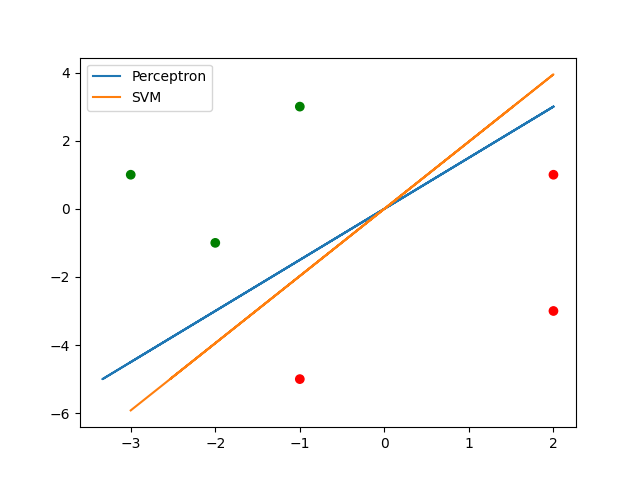
\includegraphics{code/exercise_01.png}
\end{center}
\begin{enumerate}[label=(\alph*)]
	\item	Perceptron Learning: \\
			\bigskip

			Updating vector $w=(0, 0)$ using $(x,y)=((2, 1), -1)$ \\
			$w=(-2, -1) \rightarrow w=(0, 0) + y=-1 * x=(2, 1)$ \\
			\bigskip

			Updating vector $w=(-2, -1)$ using $(x,y)=((-1, 3), 1)$ \\
			$w=(-3, 2) \rightarrow w=(-2, -1) + y=1 * x=(-1, 3)$ \\
			\bigskip

			Margin: $0.3076923076923077$
	\item	SVM Learning: \\
			\bigskip

			0.0
			$w^*: (-0.6074814098863559, 0.30790724037405226)$ \\
			Margin: $1.9555332420486629$
\end{enumerate}


\section*{Exercise 2}
\begin{enumerate}[label=(\alph*)]
	\item	$\hat{w}=\textbf{1}=(1, \dots, 1) \in \{1\}^n$ is a suitable weight vector, since $\langle \hat{w},x \rangle$ is only positive, iff $x$ contains more $1$'s than $-1$'s.
	\item	$\lambda = n$, since $\Abs{x}$ is maximum when $x$ consists of either only $1$'s or only $-1$'s. \\
			$\gamma = \frac{1}{n}$ since the margin is minimal for a $x$ which consists of an by one number off amount of $1$'s and $-1'$. Thus, $\frac{\abs{\langle w,x \rangle}}{\Abs{w}} = \frac{1}{n}$ \\
			Using Theorem 1.13 we can derive that the perceptron algorithm finds a linear separator after at most $\left(\frac{\lambda}{\gamma}\right)^2 = \left( \frac{n}{\frac{1}{n}}\right)^2 = n^4$ updates.
\end{enumerate}


\section*{Appendix}\label{appendix}
\subsection*{Code for Exercise 1}
\lstinputlisting[language=Python]{code/exercise_01.py}

\end{document}